\chapter{Research Methodology}
\label{Chapter2} % For referencing this chapter elsewhere, use \ref{Chapter3}

\section{Research design} \label{design}

\noindent In this I look at the structural foundation for running the comparative study of the Random Survival Forest \parencite{ishwaran_random_2008} and the Cox proportional hazards model \parencite{cox_regression_1972}. Central to this design is the use of \textbf{simulation studies}, to gain empirical insights into the behavior of the statistical methods across various scenarios. As \parencite{morris_using_2019} aptly puts it, "Simulation studies are used to obtain empirical results about the behavior of statistical methods in certain scenarios, as opposed to analytic results."
\\\\
\noindent This section focuses on the application of the (ADMEP) framework, formalized by \parencite{morris_using_2019}. This framework is the building block of most of the methodical parts later on in the methodology. It served as the backbone of my methodology, allowing me to produce results that "accurately" reflect the performance and effectiveness of these models.

\begin{figure}[h]
 \centering
 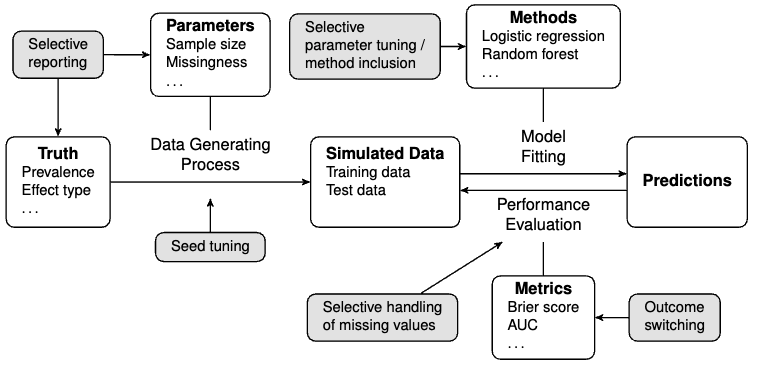
\includegraphics[scale=0.25]{Figures/METHOD_GRAPH.png}
 \caption{\parencite{pawel_pitfalls_2024} Shows a common example of a simulation study plan.}
\end{figure}

\noindent Taking inspiration from the the application of ADMEP by \parencite{pawel_pitfalls_2024}, the following sections define methods relevant in each section of the framework for later use in the methodology:

\subsection{Aims}
\begin{itemize}
\item To evaluate how effectively the Random Survival Forest and Lasso-Cox models predict survival outcomes.
\item To understand model behavior under varying conditions of data complexity and censoring rates.
\item To understand the effects of data and simulation methods. 
\end{itemize}

\subsection{Data-generating mechanisms}
\begin{itemize}
\item Simulate datasets with packages like \parencite{davidson-pilon_lifelines_2024} to introduce complexities like varying censoring rates and non-linear effects.
\item Introduce multicollinearity and various interaction effects to challenge the models' assumptions and robustness.
\end{itemize}
\
\subsubsection*{Missing Data Imputation}

As discussed in \ref{impute} we look at the methods for producing missing value imputation under the CAR and CNAR assumptions.
\\\\
\textit{Delta-adjusted Method} \parencite{jin_imputation_2024}
\begin{equation} \label{eq:deltaadjust}\lambda_{post}(t|Z_{i},X_{i}(t)) = \lambda_{\emptyset}(t|Z_{i},X_{i}(t)) = \lambda_{0}(t)\exp^{(1-\emptyset)\beta Z_{i} + \alpha X_{i}(t)}, t>C_{i}\end{equation}
\noindent The sensitivity parameter (\(\emptyset\)) represents a discounted proportion of the log-hazard ration \(\beta\) under the CNAR assumption. The method assumes that the hazard of having an event for censored subjects is multiplicatively decreased by a factor depending on the \(\emptyset\). The term \((1- \emptyset)\beta\) suggests a reduced effect of the treatment on the hazard rate post-censoring.
\\\\
\textit{Tipping point Analysis} \parencite{jin_imputation_2024}
\par \noindent This method is used to identify how much the assumption of noninformative censoring (CAR) would need to be violated for the study results to become statistically nonsignificant. It uses the delta-adjusted method's parameter \(\emptyset\) to calculate the minimum shift in \(\beta\) (log HR) needed to nullify the treatment effect.
\\\\
\textit{Jump to Reference} \parencite{jin_imputation_2024}
\begin{equation} \label{eq:jtor}\lambda_{post}(t|Z_{i},X_{i}(t)) = \lambda_{J2R}(t|Z_{i},X_{i}(t)) = \lambda_{ref}(t|X_{i}(t)) = \lambda_{0}(t)\exp^{\alpha X_{i}(t)}, t>C_{i}\end{equation}
\noindent This Method assumes that once censored, the hazard rate for a subject from the treatment group immediately aligns with that of the reference group, completely disregarding any residual effects of the treatment past the point of censoring.
\\\\
\textit{Copy Reference} \parencite{jin_imputation_2024}
\begin{equation} \label{eq:copyref}\lambda_{CR}(t|Z_{i} = 1,X_{i}(t)) = \lambda(t|Z_{i} = 0, X_{i}(t)) = \lambda_{0}(t)\exp^{\alpha X_{i}(t)} \text{for all}, t\end{equation}
\noindent This method is conservative but less so than J2R in that it assumes that if a subject in the treatment group is censored, their hazard function matches that of the reference group for the remainder of the study. It does not account for any time-specific variations in hazard that might have been influenced by the treatment before censoring.
\\\\
\textit{Censored at Random (CAR)} \parencite{jin_imputation_2024}
\par \noindent Assumes noninformative censoring where the post-censoring hazard (\(\lambda_{post}\)) is identical to the pre-censoring hazard, simplifying the imputation process.

Hazard post CAR: 
\begin{equation} \label{eq:carassmp}\lambda_{post}(t|Z_{i},X_{i}(t)) = \lambda_{0}(t)\exp^{\beta Z_{i} + \alpha X_{i}(t)}, t>C_{i}\end{equation}

Hazard post CNAR:
\begin{equation} \label{eq:cnarassmp}\lambda_{post}(t|Z_{i},X_{i}(t)) \neq \lambda_{0}(t)\exp^{\beta Z_{i} + \alpha X_{i}(t)}, t>C_{i}\end{equation}

\subsubsection*{Data Simulation}
\textit{Parametric Distribution}
\par \noindent This method is used to simulate survival times using predefined parametric distributions. The fit of each distribution to the data is tested using the one-sample Cramér-von Mises (CVM) test \parencite{thurow_how_2023}. The distribution that shows the least deviation from the data (highest p-value in the CVM test) is chosen for simulation. Parameters for these distributions are estimated using Maximum Likelihood Estimation (MLE). An Example of mixed distribution: 
\begin{equation} \label{eq:paramdist}f(x)=0.2.f_{Weibull}(\alpha,\lambda)+0.8.f_{norm}(\mu,\sigma)(x)\end{equation}
\noindent Where \(f_{Weibull(\alpha, \lambda)}\) and \(f_{norm}(\mu,\sigma)\) are the density functions for the Weibull and normal distributions, respectively.
\\\\
\textit{Kernel Density Estimation (KDE)}
\par \noindent Used to estimate by utilizing the density function of the data for simulation. The density function is estimated using the kdensity function from the \parencite{thurow_how_2023} R-package, which employs a Gaussian kernel. The Accept-reject method is used to generate random values that follow the estimated density function. Draw \((X, U)\) from the joint distribution \((X, U) ~ \left\{ (x,u):0<u<f(x)\right\}\) where X is a random variable following the estimated density f, and U is uniformly distributed between 0 and \(f(x)\). If \(u_{i} < f(x_{i})\) for a sampled \((X,U),x_{i}\) is accepted as a realization from the density function \(f\)
\\\\
\textit{Case Resampling}
\par \noindent Simulate data by resampling observed data points with replacement. Directly resample observations (ti, di) from the existing dataset of observed times and censoring indicators. \((t_{i}, d_{i})^{*}\) are drawn with replacement from \(\left\{ (t_{1}, d_{1}) \dots (t_{n}, d_{n})\right\}\)
\\\\
\textit{Conditional Bootstrapping}
\par \noindent To simulate data using bootstrapping that accounts for censoring, this helps sample censor times. For censored observations, censoring times are carried over to the simulated data. For uncensored observations, new censoring times are sampled based on the conditional distribution of censoring times given they are greater than the observed event time. Censoring Time for censored data: \(c_{i}^{*} = t_{i}\) for censored observation. Censoring Time for uncensored data: \(c_{i}^{*}\) is sampled from \(G_{i}(c) = \frac{G(c)-G(t_{i})}{1-G(t_{i})}\) where \(G\) is the distribution function of censoring times and \(t_{i}\) is the observed event time. Event times \(t^{*}_{oi}\) are sampled from the observed event times with replacement. \parencite{thurow_how_2023} Show that the reconstruction of reliable benchmark data sets is meticulously reconstructed from published Kaplan-Meier plots and other vital statistics like hazard ratios and p-values from log-rank tests. The data sets, particularly those with non-crossing survival curves, demonstrate high fidelity to the original data, proving them to be excellent resources for subsequent model evaluations.
\subsubsection*{Synthetic Data Generation}
\noindent \parencite{norcliffe_survivalgan_2023} Employ several metrics to assess synthetic survival data according to the real dataset. They help identify and correct biases in synthetic data to better align with real-world data, enhancing the credibility of survival analysis models. The optimism metric assesses whether the synthetic data is over-optimistic or over-pessimistic compared to real data by comparing the expected lifetimes derived from Kaplan-Meier (KM) plots.
\begin{equation} \label{eq:optimisim}\text{Optimism} = \frac{1}{T} \int_{0}^{T}(S_{Syn}(t)-S_{Real}(t))dt\end{equation}
\noindent Where \(S_{Syn}(t) and S_{Real}(t)\) are the synthetic and real Kaplan-Meier survival functions respectively, and T is the latest time point available. The optimism metric ranges between -1 and 1, where values closer to 0 indicate accurate lifetime predictions, positive values suggest over-optimism, and negative values indicate over-pessimism. The short-sightedness metric quantifies how much earlier synthetic data, discontinues providing predictions compared to real data, reflecting potential censorship in the synthetic modeling.
\begin{equation} \label{eq:ssmetric}\text{Short-Sightedness} = \frac{T_{Real}-T_{Syn}}{T_{Real}}\end{equation}
\noindent Here, \(T_{Syn} and T_{Real}\) are the end times of the synthetic and real Kaplan-Meier plots, respectively. This metric ranges from 0 to 1, where 0 indicates no censorship issues and 1 indicates complete short-sightedness in the synthetic data predictions. Lastly, the Kaplan-Meier divergence measures the overall divergence between the synthetic and real KM curves across the observed time, providing a comprehensive measure of similarity between the two datasets.
\begin{equation} \label{eq:kmdiverge}\text{KM Divergence} = \frac{1}{T}\int_{0}^{T}|S_{Syn}(t)-S_{Real}(t)|dt\end{equation}
\noindent This formula calculates the mean absolute difference between the synthetic and real survival functions over time, scaled by the total duration observed. The KM divergence values range from 0 to 1, where 0 indicates perfect matching KM curves and 1 represents the maximum possible difference.

\subsection{Methods}
\begin{itemize}
\item Random Survival Forest: Implement using a combination of proposed packages in \ref{methods}, tuning tree-related parameters.
\item Lasso-Cox Model: Use a combination of the proposed packages in \ref{methods} for implementing Cox regression with Lasso regularization, optimizing the regularization strength and model complexity. 
\item Explore integration effects from the different packages.
\end{itemize}

\subsubsection*{Cox Proportional Hazards Model}
The proposition consists of covariates, known as attributes regarding a unit in a distribution of data, which is associated with a coefficient \(\beta\) scaling the impact of said covariates; this product is then bound by the baseline hazard \(h_{0}(t)\).
\begin{equation} \label{eq:cox}h(t|X) = h_0(t) \exp(\beta_1 X_1 + \beta_2 X_2 + \ldots + \beta_n X_n)\end{equation}
An assumption of the Cox model is the proportional hazards assumption, suggesting that the hazard ratios for different covariates remain constant over time we see this for two events observations. This is an operational Assumption and a limitation as this is not always true for survival data. 
\begin{equation} \label{eq:coxph}\frac{h(t|X_1)}{h(t|X_2)} = \frac{h_0(t) \exp(\beta^T X_1)}{h_0(t) \exp(\beta^T X_2)} = \frac{\exp(\beta^T X_1)}{\exp(\beta^T X_2)} = \exp(\beta^T (X_1 - X_2))\end{equation}
The model can handle censoring, by adjusting the likelihood function for observations where event occurrence did not happen in a particular continuous time frame, and by maximizing the likelihood of all observed events, it is possible to estimate the coefficients that could work the best under the Cox formulation.
\begin{equation} \label{eq:coxlikely}L(\beta) = \prod_{i: \delta_i = 1} \frac{\exp(\beta^T X_i)}{\sum_{j \in R(t_i)} \exp(\beta^T X_j)}\end{equation}

\subsubsection*{Lasso Regularisation}
\noindent The Lasso technique \parencite{tibshirani_regression_1996}, a regression analysis method introduced to address specific limitations of Ordinary Least Squares (OLS) estimation, is particularly beneficial in scenarios with a large number of predictors or high collinearity among them which would mean that models could produce inflated variance scores, and cause impaired interpretability. Lasso optimizes prediction accuracy and enhances model interpretability by employing a shrinkage process that can set certain coefficients to zero effectively, thus performing variable selection.
\begin{equation} \label{eq:lasso}\hat{\beta}^{lasso} = \arg \min_{\beta} \left\{ \frac{1}{2N} \sum_{i=1}^{N} (y_i - \beta_0 - \sum_{j=1}^{p} X_{ij}\beta_j)^2 \right\}\end{equation}
bound by,
\begin{equation} \label{eq:lassobound}\sum_{j=1}^{p} |\beta_j| \leq t.\end{equation}
\noindent \parencite{freijeirogonzalez_critical_2022} The inclusion of the regularisation term, is crucial as it allows for the reduction of model complexity by penalizing the magnitude of the coefficients, which promotes sparser models. This sparsity is instrumental in enhancing interpretability by isolating only the most significant predictors that contribute to the dependent variable. The objective function of LASSO is convex for \(l_{1}\) norm, which simplifies finding the global minimum. Multiple optimal solutions might exist, especially when the number of predictors \(p\) exceeds the number of observations \(n\). \parencite{freijeirogonzalez_critical_2022} LASSO introduces bias in the coefficients to achieve lower variance and better model parsimony. Consistent under conditions like the irrepresentable condition, crucial for variable selection. Bias Correction achieved via,
\begin{equation} \label{eq:lassobais}\hat{\beta}_{j}^{LASSO}=sign(\hat{\beta}_{j}^{OLS})(|\hat{\beta}_{j}^{OLS}| - \lambda)_{+}\end{equation}

\subsubsection*{Random Survival Forest}
\noindent Random survival forests \parencite{ishwaran_random_2008} are an extension of random forests, which can handle right-censored data and aim to estimate the appropriate survival function. Consisting of an ensemble of trees \parencite{ishwaran_random_2008}, which are grown from a bootstrap sample, and each node of underlying trees, consists of specific covariates due to a random selection of features for splits in each tree.
\\\\
\noindent Per node splitting criteria are conditional to survival time and censoring, whereby node “impurity” \parencite{ishwaran_random_2008} is determined by the survival differences. Methods like log-rank, conservation of events splitting rule, and random log-rank are used. Terminal nodes are the result of saturated splitting criteria, with each endpoint having d-dimensional covariates of the individuals encapsulated. 
\\\\
\noindent A key component of the model is the conservation of events principle, which is used to define a type of predicted outcome, namely ensemble mortality, which is derived from the cumulative hazard function (CHF) using the Nelson-Aalen estimator in the original paper by \parencite{ishwaran_random_2008}. 
\\\\
\noindent Terminal nodes or nodes at the end of tree branches all share the estimated hazard function. Another key concept is the out-of-bag (OOB) samples which act as a validation subset \parencite{ishwaran_random_2008}. 
\\\\
\noindent The OOB error is calculated on the ensemble survival function of the observed data using metrics like concordance (C-index). Used for estimating prediction error and model performance without a separate test data set. Each tree's error is calculated using data not included in its training set (out-of-bag). Prediction error metrics, like the concordance index which calculates the permissible pairs per node and OOB prediction error, are used for accuracy metrics. 

\begin{equation} \label{eq:ooberror}
\hat{\Lambda}_{oob}(t,x_{i}) = \frac{1}{\sum_{b=1}^{B}I(x_{i}\in L^{b}_{oob})}\sum_{b=1}^{B}I(x_{i}\in L^{b}_{oob})\hat{\Lambda}_{b}(t,x_{i})
\end{equation}


\subsection{Estimands}
\begin{itemize}
\item Focus on estimations, like survival functions, hazard ratios, etc. for both models and survival probabilities at specified time points.
\item Bootstrap samples to build confidence intervals for key estimands, ensuring the robustness of the findings.
\item Analyze feature importance in RSF and assess how Lasso regularization affects the selection of covariates in the Cox model.
\end{itemize}

\subsubsection*{Lasso Penalised Cox Proportional Hazards}
The log partial likelihood for the Cox model, as given by:

\begin{equation} \label{eq:likelihood}l(\beta) = \sum_{i:\delta_{i}=1} \left[ \beta^{T}x_{i} - \log{\sum_{j:t_{j}\ge t_{i}} \exp(\beta^{T}x_{j})} \right]\end{equation}

\noindent Which provides a measure of how well the model's predicted hazards match the observed data. Here, \(\delta\) indicates whether an event (e.g., failure, death) was observed at time \(t_{i}\). 

\subsubsection*{Random Survival Forests}
Random forests are adapted for survival analysis by modifying how predictions are aggregated to handle censored data effectively. Forest survival function estimator:
\begin{equation} \label{eq:rsfestimator}\hat{\Lambda}(t, x_{0}) = \frac{1}{B} \sum_{b=1}^{B} \hat{\Lambda}_{b}(t,x_{0})\end{equation}
Survival function:
\begin{equation} \label{eq:survrsf}S(t,x_{0}) = \exp^{-\hat{\Lambda}(t,x_{0})}\end{equation}

\noindent Variable importance (VI) \parencite{pham_springer_2023} in random forests is used to rank variables based on their contribution to prediction accuracy. It is assessed by looking at each predictor variable in the sample and assessing the impact on prediction error, an increase in error indicating importance. Different random forest settings can yield different importance rankings due to the model's sensitivity to the configuration. VI is shown by \parencite{pham_springer_2023}:
\begin{equation} \label{eq:vinorm}
VI(j) = \frac{1}{B}\sum_{b=1}^{B}(\frac{Err(j)_{b}}{Err_{b}}-1)
\end{equation}

\noindent VI Adaptation:
\begin{equation} \label{eq:viadapt}VI(j) = \frac{1}{B}\sum_{b=1}^{B}(\frac{Err(j|Z)_{b}}{Err_{b}}-1)\end{equation}

\noindent This adaptation \ref{eq:viadapt} addresses correlations \parencite{pham_springer_2023} by conditioning on other related variables. This accounts for the influence of correlated predictors by adjusting the variable importance calculation.


\subsection{Performance measures}
\begin{itemize}
\item Use statistical tests, like the C-index, and integrated Brier score to compare the RSF and Lasso-Cox model's performance metrics, like predictive accuracy, discrimination, and calibration across time.
\item Conduct sensitivity analysis to explore the impact of model parameters on their performance.
\item Apply graphical methods like Kaplan-Meier curves to visualize survival estimates against actual outcomes.
\end{itemize}

\subsubsection*{C-Index}
\noindent The C-index \parencite{qi_effective_2023}, serves as a crucial statistical measure in evaluating the effectiveness of survival models. This index assesses how well these models predict the sequence of patient outcomes based on their respective risk assessments. It is defined as the ratio of pairs of subjects (deemed "comparable") for which the model's predictions and actual outcomes are consistent in terms of event sequence. "Comparable" refers to pairs where the event sequence, i.e., who encountered the event first, can be established.
\begin{equation} \label{eq:cindex}C\text{-index} = \frac{\sum_{i,j} \mathbf{1}(t_i < t_j) \cdot \mathbf{1}(\eta_i > \eta_j) \cdot \delta_i}{\sum_{i,j} \mathbf{1}(t_i < t_j) \cdot \delta_i}\end{equation}
\noindent In this formula, \(\mu_{i}\) is the risk score for unit i, and \(\delta_{i}\) indicates whether an event occurred (1 if it did, 0 otherwise)
\subsubsection*{Brier Score and Integrated Brier Score}
\textit{Brier score} is a measure used to evaluate the accuracy of probabilistic predictions. It is essentially the mean squared error \parencite{qi_effective_2023} between the observed outcomes and the predicted probabilities at a specific time \(t^{*}\).
\begin{equation} \label{eq:bs}BS_{t^*}(VU, \hat{S}(t^* | \cdot)) = \frac{1}{|VU|} \sum_{[\tilde{x}_i, d_i] \in VU} (I[d_i \leq t^*] - \hat{S}(t^* | \tilde{x}_i))^2\end{equation}
\noindent Where, \(VU\) is the validation set, \(\hat{S}(t^* | \cdot))\) is the predicted survival probability at \(t^{*}\) and \(I[d_i \leq t^*]\) is the event indicator.
\\\\
\noindent \textit{Integrated Brier Score (IBS)} extends the Brier score across a range of times, providing a measure of model accuracy over time. In other words, it is the expectation of the Brier scores calculated at each time point within a specified interval.
\begin{equation} \label{eq:ibs}IBS(\tau, VU, \hat{S}(\cdot | \cdot)) = \frac{1}{\tau} \int_0^{\tau} BS_t(VU, \hat{S}(t | \cdot)) \, dt\end{equation}
\noindent Where, \(\tau\) is the biggest event period, \(BS_{t}\) is the brier score at time t.
\subsubsection*{1-Calibration}
\noindent 1-Calibration, also known as Hosmer-Lemeshow calibration, is a test used to evaluate model calibration at a specific time point \(t^{*}\) \parencite{haider_effective_2018}.
It works by sorting all subjects for the predicted probabilities at time \(t^{*}\). These probabilities are then grouped into a predefined number of groups or bins (typically 10). For each bin, number of events is determined based on the predicted probabilities, and this is compared to the actual number of events that occurred \parencite{qi_effective_2023}.

\begin{equation} \label{eq:c1}\text{HL}(VU, \hat{S}(t^* | \cdot)) = \sum_{j=1}^B \frac{(O_j - n_j \bar{p}_j)^2}{n_j \bar{p}_j (1 - \bar{p}_j)}\end{equation}
\noindent Where, \(B\) is the number of bins, \(O_{j}\) is the observed number of events in bin j, \(\hat{p}_{j}\) is the average predicted probability in bin j. 

\subsubsection*{D-Calibration}
\noindent D-Calibration \parencite{haider_effective_2018} extends the concept of 1-calibration over a range of time points or across different distributions of time points, providing a more comprehensive measure of a model's accuracy.

% \begin{equation} \label{eq:dc}D_{\Theta}([a, b]) = \{[x_i, d_i, \delta_i = 1] \in D | \hat{S}_{\Theta}(d_i) \in [a, b]\}\end{equation}

\subsubsection*{Mean Absolute Error}
\par \noindent \textit{Mean Absolute Error} (MAE) (Uncensored) is the simplest form of MAE variants indicated by \parencite{qi_effective_2023}, it is calculated by taking the non negative value difference between the predicted and actual event times for uncensored subjects only. It does not consider censored data, which may introduce bias when censoring rate is frequent.
\begin{equation} \label{eq:rmae}
RMAE (\hat{t}_i, t_i, \delta_i = 1) = |t_i - \hat{t}_i|
\end{equation}
\par \noindent \textit{MAE-Hinge} variant \parencite{qi_effective_2023} considers only the cases where the estimated time is sooner than the actual cesonsoring time. It is somewhat optimistic as it assigns zero error to predictions that are later than or equal to the censoring time. Applied when the actual event time is censored \(\delta (i =0)\)
% \begin{equation} \label{eq:maehinge}
% RMAE\text{-hinge}(\hat{t}_i, t_i, \delta_i = 0) = \max(t_i - \hat{t}_i, 0)
% \end{equation}
\par \noindent \textit{"MAE-Margin"} \parencite{qi_effective_2023} uses a "margin time" for induvivual censored units, estimated using a non-parametric method (Kaplan-Meier estimator). This "margin time" is treated as an adjusted event time, creating a more informed guess for censored individuals.
\begin{equation} \label{eq:maemargin}
\text{Error for censored subjects:} \quad \omega_i[(1 - \delta_i) \cdot \text{emargin}(t_i) + \delta_i \cdot t_i] - \hat{t}_i
\end{equation}
\noindent \parencite{qi_effective_2023} shows that \(w_{i} = 1-S_{KM}(t_{i})\) confidence weight based on the Kaplan-Meier estimator \(emargin(t_{i})=t_{i}+\int_{t_{i}}^{\infty} S_{KM}(D)(t)/S_{KM}(D)(t_{i})\) margin time.
\\\\
\noindent \textit{"MAE-IPCW-D"} ("Inverse Probability Censoring Weight" - Difference) adapts the "IPCW" method to MAE by re-allocating the weights of censored subjects to those with known outcomes, using the estimated time of the event for calculations.
\par \noindent Then, \textit{RMAE-IPCW-T} is calculated similarly to RMAE-IPCW-D, but using eIPCW  for censored subjects. MAE-PO (Pseudo-Observation) utilizes pseudo-observations that estimate the impact of each data point on the overall survival time estimate. 
\begin{equation} \label{eq:maepsuedo}e_{pseudo-obs}(t_i, D) = N \cdot \hat{\theta} - (N - 1) \cdot \hat{\theta}_{-i}\end{equation}
\par \noindent \(\theta\) and \(\hat{\theta}\) are unbiased survival time estimators with and without the ii-th subject. The pseudo-observation is treated as an observed event time for MAE calculations.

% \subsubsection*{Ranked Probability Score}
% Ranked probability score \parencite{yanagisawa_proper_2023} extends the concept of the Brier Score to multi-class problems by considering the cumulative probability distributions. It evaluates the accuracy of predictions across all possible categorical outcomes, making it highly useful for discrete classification tasks in survival analysis.
% \begin{equation} \label{eq:ranked}S_{\text{RPS}}(\hat{F}, y) = \sum_{i=1}^{B-1} S_{\text{Binary-Brier}}(\hat{F}, y; \zeta_i)\end{equation}

\subsubsection*{Logarithmic Score}
The Logarithmic Score \parencite{yanagisawa_proper_2023} is used for models that predict the entire probability distribution of the event times. It rewards models that assign higher probabilities to the events that occur. It assesses the logarithm of the predicted probabilities assigned to the true outcome intervals, promoting models that are confident and correct about their predictions.
\begin{equation} \label{eq:logscore}S_{\text{Log}}(\hat{F}, y; \{\zeta_i\}) = -\sum_{i=0}^{B-1} 1(\zeta_i < y \leq \zeta_{i+1}) \log(\hat{F}(\zeta_{i+1}) - \hat{F}(\zeta_i))\end{equation}

\subsubsection*{Cross-Validation}
\parencite{harrell__regression_2015} Cross-validation is a resampling technique used to evaluate the generalizability of a statistical model by systematically partitioning the dataset into training and validation subsets. The most granular form, leave-one-out cross-validation (LOOCV), omits one observation at a time from the dataset of size $n$, fits the model on the remaining $n-1$ observations, and uses the excluded observation to test the model's performance. The process is repeated $n$ times, yielding an average accuracy metric, typically denoted by $\hat{\theta} = \frac{1}{n} \sum_{i=1}^{n} \theta_i$, where $\theta_i$ is the performance metric for the $i$-th iteration. Grouped cross-validation, a more practical alternative, divides the data into $k$ subsets, using $k-1$ subsets for model training and the remaining subset for validation, iterating this process $k$ times. Although cross-validation mitigates some issues of data-splitting, it is computationally expensive, often requiring numerous repetitions (e.g., 200+ iterations) to stabilize accuracy estimates. Moreover, the method may not fully capture the variability of variable selection, as subsets tend to produce similar feature sets. Additionally, cross-validation does not validate the model on the full dataset, which can lead to an underestimation of the model's overall predictive power. To address potential overfitting, a randomization method can be employed, where the response variable $Y$ is randomly permuted, and the model's predictive accuracy on this randomized data is compared to its performance on the original data, with significant deviations indicating possible overfitting.

\section{Data}
\noindent For my research, I utilized SurvSet, an open-source repository specifically designed for time-to-event (T2E) analysis. SurvSet provides a standardized collection of 76 datasets, primarily focused on biomedicine, that are formatted consistently for easy preprocessing and analysis. This makes it an ideal source for benchmarking machine learning (ML) algorithms in survival analysis.
\\\\
\noindent To understand the specifics of each dataset within SurvSet, the repository provides a clear and consistent structure. Each dataset is accompanied by a unique ds\_name and metadata that detail its characteristics, such as whether it includes time-dependent covariates, the number of features, and the types of variables (numerical or categorical). The SurvLoader class allows users to easily load any dataset and access this metadata, along with a reference URL that offers additional context and explanations for the columns. This structure ensures that researchers can quickly grasp what each dataset is used for and how it can be applied in survival analysis or machine learning benchmarking.
\\\\
\noindent SurvSet organizes datasets using a SurvLoader class, which simplifies loading and accessing data. Each dataset includes core columns like \texttt{pid} (unique ID), \texttt{event} (whether the event occurred), and \texttt{time} (time to event or censoring). Features are clearly marked as either numerical (num\_\{\}) or categorical (fac\_\{\}), ensuring a smooth integration with various ML algorithms. This consistent structure across all datasets in SurvSet made it my go-to source for accurate and reliable survival analysis in my project.
\\\\
\noindent Furthermore, when selecting the dataset censoring levels, FAIR principles \parencite{wilkinson_fair_2016}, reproducibility by assessing data simulation accuracy similar to the KM-Divergence metric used by \parencite{norcliffe_survivalgan_2023} are all important considerations. Utilizing this approach voids the need to carefully assess the ethical implications of using the datasets as these datasets should be under public licensed availability. Lastly, I don't foresee data preprocessing steps, being necessary, as DGM for simulation are commonly categorized as postprocessing \parencite{jin_imputation_2024}.


\section{Methods} \label{methods}
\subsection{Exploratory Analysis}
Exploratory Data Analysis (EDA) is a crucial first step to discover key considerations for contributing covariates and potential implications. In line with the principles outlined in \parencite{harrell__regression_2015}, this EDA focuses on a detailed examination of the survival data's structure, distribution, and key features such as outliers, missing values, and multicollinearity, that could impact the performance and validity of our regression models.
\\\\
\noindent \textit{Data Overview} The dataset's dimensions, including the number of rows and columns, are first examined to understand its size. Next, we verify the data types of each column (such as time, event, and covariates) to ensure they are appropriate for analysis. Additionally, we identify and assess missing values across the dataset, visualizing these patterns using a heatmap or matrix plot to uncover any systematic issues.
\\\\
\noindent \textit{Target Variable Analysis (Survival Time and Event Status)} For the survival time (time), summary statistics such as mean, median, range, and standard deviation are calculated. We then plot the distribution of survival times using a histogram or density plot to visualize these statistics. For the event status (event), the proportion of events versus censored cases is determined and visualized through a bar chart to understand the distribution of event occurrences.
\\\\
\noindent \textit{Univariate Analysis of Covariates} In the univariate analysis, summary statistics for each numerical covariate are calculated, including the mean, median, minimum, and maximum values. These statistics are further visualized through histograms or density plots to assess their distributions. For categorical covariates, we count the frequency of each category and visualize the distribution using bar charts.
\\\\
\noindent \textit{Bivariate Analysis} To explore relationships between survival time and covariates, scatter plots are created for numerical covariates, while box plots are used to compare survival times across different levels of categorical covariates. For the event status versus covariates, bar charts or stacked bar charts are used to visualize the distribution of event status across categorical covariates. Violin plots or box plots are also employed to assess the distribution of numerical covariates within each event status, such as comparing values for censored versus event occurred.
\\\\
\noindent \textit{Censoring Analysis} Censoring is analyzed by calculating and visualizing the overall censoring level in the dataset, expressed as the percentage of censored observations. Additionally, we explore how censoring is distributed across different covariates by creating grouped bar charts or box plots.
\\\\
\noindent \textit{Correlation Analysis} For numerical covariates, a correlation matrix is calculated and visualized using a heatmap to identify relationships between variables. For categorical covariates, relationships with numerical covariates are explored using point-biserial correlations, while Chi-square tests are used where appropriate to examine relationships between categorical variables.

\subsection{Data Processing and Simulation}

\subsubsection*{Data Processing}
\subsubsection*{Simulation}
For the simulation, I utilized the Synthcity library \parencite{qian_synthcity_2023}. Synthcity is an open-source package designed for generating and evaluating synthetic data across various data modalities, including static data, regular and irregular time series, and censored data. It provides a unified platform for innovative use cases in machine learning fairness, privacy, and data augmentation. The library was chosen for its comprehensive support of survival analysis and synthetic data generation, making it an ideal tool for this study.
\begin{figure}[h]
    \centering
    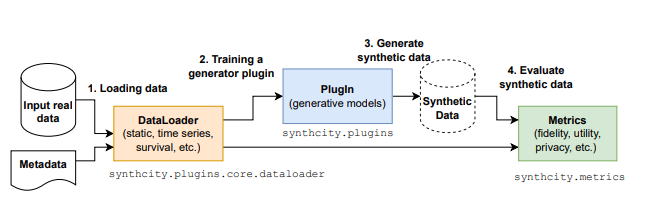
\includegraphics[scale=0.68]{Figures/SynthCity.png}
    \caption{\parencite{qian_synthcity_2023} Simulation Pipeline.}
\end{figure}

\noindent Among the various generative models available in Synthcity, I focused on the use of Survival GAN and Survival VAE. These methods were selected based on previous explorations and their proven ability to handle the complexities of survival data. Survival GAN is particularly effective in generating high-fidelity data with the capability to preserve the underlying distribution, while Survival VAE offers a robust framework for capturing the latent structure of the data, making it suitable for the simulation of censored survival datasets.
The simulation pipeline is designed to effectively generate synthetic survival data that mirrors real-world datasets, following the structured process provided by Synthcity. The design integrates several key components and classes from Synthcity, ensuring a comprehensive approach to data generation and evaluation.
\\\\
\noindent \textit{Data Loading.} \parencite{qian_synthcity_2023} The first step in the pipeline involves loading the real survival datasets using the \texttt{DataLoader} class from Synthcity. The \texttt{DataLoader} processes the survival times, censoring indicators, and covariates. Furthermore The \texttt{DataLoader} provides validation for censored observations, ensuring that the survival times and event indicators are correctly aligned for downstream modeling. Metadata, such as identifying sensitive features or specifying outcome variables, can be included.
\\\\
\noindent \textit{Model Training.} The \texttt{Plugin} class is used to instantiate these models, allowing for straightforward training and application. The training is conducted using the \texttt{fit()} method of the \texttt{Plugin} class.
\\\\
\noindent \textit{Synthetic Data Generation.} Once the models are trained, the \texttt{generate()} method of the \texttt{Plugin} class is used to produce synthetic datasets. The design considerations at this stage include:
\\\\
\noindent \textit{Evaluation of Synthetic Data.} The final component of the pipeline involves evaluating the synthetic data using the \texttt{Metrics} class provided by Synthcity. The design focuses on several key evaluation aspects:
\begin{itemize}
    \item Fidelity Metrics: The \texttt{Metrics} class is utilized to assess how closely the synthetic data resembles the original data. Metrics such as distributional similarity and survival curve alignment are critical for determining data fidelity. 
    \item Utility Evaluation: The utility of the synthetic data for downstream tasks is tested by applying standard machine learning models to the generated data and comparing performance against models trained on real data. 
    \item Privacy Considerations: Privacy is a major concern in synthetic data generation. The \texttt{Metrics} class includes tools to evaluate the privacy of the synthetic data, such as assessing the risk of re-identification or leakage of sensitive information. 
\end{itemize}

\subsection{Survival Analysis: Model Application and Evaluation}

\noindent For this section I outline the steps For running the models on the loaded and preperad data. The libraries utilized in the study consist of:

\begin{table}[h]
\begin{tabularx}{\textwidth}{|X|X|}
\hline
Library/Method & Description \\
\hline
Auton-survival \parencite{nagpal_auton-survival_2022} & Provides tools for survival analysis including implementations of advanced machine learning models like DeepSurv and Cox-Time. \\
\hline
scikit-survival \parencite{sebastian_polsterl_scikit-survival_2023} & Extends scikit-learn \parencite{scikit-learn} to handle survival analysis, enabling use of Cox regression models with extensions such as Lasso. \\
\hline
lifelines \parencite{davidson-pilon_lifelines_2024} & Popular library for survival analysis that includes Kaplan-Meier, Nelson-Aalen, and Cox models, among others. \\
\hline
\end{tabularx}
\caption{Libraries to be used during research}
\label{tab:libs}
\end{table}

\subsubsection*{Cox Proportional Hazards (CoxPH) Model}

\paragraph*{Model Fitting}
\begin{itemize}
    \item Fit the CoxPH model using the \texttt{lifelines} library.
    \item Check the proportional hazards assumption with \texttt{lifelines.check\_assumptions()}.
\end{itemize}

\paragraph*{Lasso Regularization}
\begin{itemize}
    \item Apply Lasso regularization (L1 penalty) during the fitting process to perform feature selection by shrinking coefficients of less important covariates to zero.
    \item Use the \texttt{lifelines.CoxPHFitter(penalizer=penalty)} with a chosen penalty term to control the amount of regularization applied. 
    \item Use metrics like the cross-validation score
\end{itemize}

\paragraph*{Effect of Lasso on Model Performance}
\begin{itemize}
    \item Lasso regularization can help reduce model complexity by selecting a subset of relevant covariates, which may improve the interpretability and generalization of the CoxPH model.
    \item Evaluate the impact of Lasso on model performance by comparing the concordance index (C-index) and analyzing the selected covariates.
\end{itemize}


\paragraph*{Survival Curve Prediction}
\begin{itemize}
    \item Predict survival function using \texttt{predict\_survival\_function()}.
    \item Plot survival curves for different covariate profiles.
\end{itemize}


\paragraph*{Covariate Contribution Analysis}
\begin{itemize}
    \item Use \texttt{lifelines.plot\_covariate\_groups()} to visualize covariate impact.
    \item Create boxplots to analyze covariate effects on the hazard ratio.
\end{itemize}

\paragraph*{Model Evaluation}
\begin{itemize}
    \item Compute concordance index (C-index) for model performance.
    \item Evaluate model performance across different levels of censoring.
    \item Perform stratified analysis based on different censoring levels.
    \item Validate model with cross-validation or bootstrap methods.
\end{itemize}

\paragraph*{Assumption Checking}
\begin{itemize}
    \item Validate proportional hazards assumption with Schoenfeld residuals.
    \item Explore any violations and consider adjustments like stratified models.
\end{itemize}

\subsubsection*{Random Survival Forest (RSF) Model}

\paragraph*{Model Fitting}
\begin{itemize}
    \item Fit the RSF model using a the library \texttt{scikit-survival}.
    \item Tune model parameters (e.g., number of trees, max depth).
\end{itemize}

\paragraph*{Survival Curve Prediction}
\begin{itemize}
    \item Predict survival curves for each observation.
    \item Aggregate and plot survival probabilities across different covariate profiles.
\end{itemize}

\paragraph*{Variable Importance}
\begin{itemize}
    \item Analyze covariate importance using the \texttt{variable\_importance\_} attribute.
    \item Visualize importance scores using Logarithmic plot for identifing contributers.
\end{itemize}

\paragraph*{Model Evaluation}
\begin{itemize}
    \item Evaluate model using out-of-bag (OOB) score or concordance index.
    \item Evaluate model performance across different levels of censoring.
    \item Analyze performance under different levels of censoring.
    \item Validate model with cross-validation or bootstrap methods.
\end{itemize}

\paragraph*{Comparison with CoxPH}
\begin{itemize}
    \item Compare survival curves from both models for specific covariate profiles.
    \item Analyze differences, especially in cases with high censoring or non-proportional hazards.
\end{itemize}

\section{Limitations} \label{methlim}
A massive limitation is that the research is tightly coupled, meaning the phases are strictly dependent on each other. This is an antipattern, \parencite{joshi_beginning_2016}, which should be planned to accommodate any failures during any of the research phases. In cases where results do not converge, or the interpretation is wrong, the tightly coupled nature of the research will also affect the preceding stages. Lastly the computation time, within the modern setting should not be a hindrance but the combination of multiple computational components like the DGM and the model execution and results evaluation, is important to take caution. 

\section{Ethical Considerations}
Ethical clearance would not be a component of this study, as the only real data that would be used, will only be selected from open source, or publicly available (public licensing) sources. Due to the nature of the topic, being closely related to sensitive information, it will be an important point of order to note in the case that results indicate or underscore ethical implications.
